%!TEX root = FHI-aims.tex
\section{Many-Body Dispersion (MBD) energy}
The non-local many-body dispersion (MBD) or correlation energy is computed using a system of coupled atomic response functions~\cite{MBD,QHORPA}. 
\begin{figure}[h]
\begin{center}
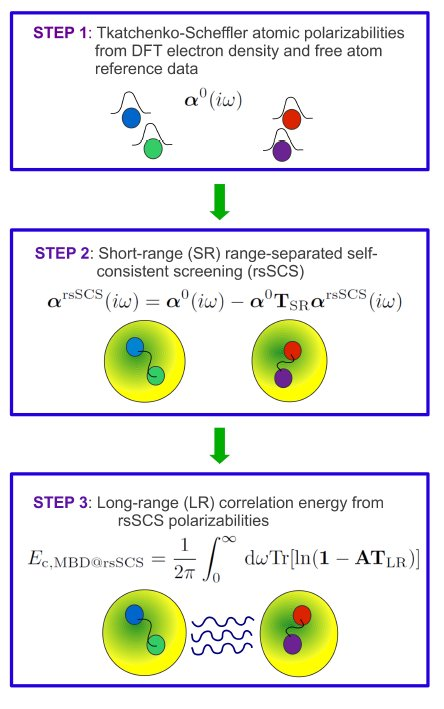
\includegraphics[scale=0.6,trim=0cm 0cm 0cm 0cm]{MBD.jpg}
\end{center}
\caption{Schematic description of the MBD@rsSCS method.} 
\label{mbdmethodfigure}
\end{figure}
The MBD method implemented in FHI-aims is the so-called range-separated MBD@rsSCS method~\cite{MBD,QHORPA}. 
The dynamic polarizability $\alpha(i\omega)$ as a function of imaginary frequency for a molecule or extended system is obtained as a solution to the self-consistent screening equation using a regularized dipole potential. The standard output of FHI-aims contains the upper triangular part of the dynamic polarizability tensor: 
\begin{verbatim}
| Many-Body Dispersion (MBD@rsSCS) energy
| Dynamic polarizability of unit cell alpha(iw)(bohr^3)
|---------------------------------------------------------------------------
| omega(Ha)   XX         YY         ZZ         YZ         XZ         XY
| 0.000000  0.717E+04  0.724E+04  0.609E+04  0.180E+01  0.752E+01  0.224E+00
| 0.039290  0.704E+04  0.711E+04  0.599E+04  0.175E+01  0.762E+01  0.222E+00
| 0.118358  0.616E+04  0.623E+04  0.529E+04  0.141E+01  0.816E+01  0.201E+00
\end{verbatim}
Furthermore, the atom projected static polarizability $\alpha(0)$ and vdW $C_{6}$ coefficient for each atom in a system are given as follows:
\begin{verbatim}
|---------------------------------------------------------------------------
| Partitioned C6 (hartree bohr^6) | alpha(bohr^3)  of atom in unit cell
|---------------------------------------------------------------------------
| ATOM   1  Zn  189.850551         30.849981
| ATOM   2  Zn  194.746383         31.378482
| ATOM   3  O   10.645313          2.411834
| ATOM   4  O   10.522485          2.335995
\end{verbatim}
Please note that the above values are derived using a range-separated dipole potential. For more technical details see Refs.~\cite{MBD,QHORPA}.

The forces or gradients for MBD@rsSCS method are available via numerical finite differences. They work for both cluster as well as periodic geometries.

\subsection*{Tags for general section of \texttt{control.in}:}

\keydefinition{many\_body\_dispersion}{control.in}
{
  \noindent
  Usage: \keyword{many\_body\_dispersion} \\[1.0ex]
  Purpose: Calculates the MBD@rsSCS energy for a given xc functional (available for PBE, PBE0, and HSE functionals).
\\[1.0ex]
}

\keydefinition{mbd\_scs\_vacuum\_axis}{control.in}
{
  \noindent
  Usage: \keyword{mbd\_scs\_vacuum\_axis} \option{flag flag flag} \\[1.0ex]
  Purpose: This keyword specifies direction of the vacuum region in case of a low-dimensional system.\\
  Default: No vacuum \keyword{mbd\_scs\_vacuum\_axis} \texttt{.false.  .false.  .false.} \\
  For example, in the case of {\it periodic} slab along $xy$ directions the keyword\\
  \keyword{mbd\_scs\_vacuum\_axis} \texttt{.false.  .false.  .true.} is needed to specify  
  $z$ as vacuum direction in MBD/SCS calculation.
}

\keydefinition{mbd\_cfdm\_dip\_cutoff}{control.in}
{
  \noindent
  Usage: \keyword{mbd\_cfdm\_dip\_cutoff} \option{value} \\[1.0ex]
  Purpose: Radius used to integrate the dipole field in a {\it periodic} MBD calculation (internal default value =100.0 Angstrom)
}

\keydefinition{mbd\_scs\_dip\_cutoff}{control.in}
{
  \noindent
  Usage: \keyword{mbd\_scs\_dip\_cutoff} \option{value} \\[1.0ex]
  Purpose: Radius used to integrate the dipole field in a {\it periodic} SCS calculation (internal default value =120.0 Angstrom) 
}
\keydefinition{mbd\_supercell\_cutoff}{control.in}
{
  \noindent
  Usage: \keyword{mbd\_supercell\_cutoff} \option{value} \\[1.0ex]
  Purpose: Radius used to construct the supercell in {\it periodic} MBD@rsSCS calculations. (internal default value = 25 Angstrom)
  NOTE: The convergence with respect to the value of \keyword{mbd\_supercell\_cutoff} must be carefully tested for periodic systems with low symmetry.
}


\keydefinition{mbd\_inversion\_method}{control.in}
{
  \noindent 
  Usage: \keyword{mbd\_inversion\_method} \option{type} \\[1.0ex]
  Purpose: Algorithm used to solve the self-consistent screening (rsSCS) problem.\\[1.0ex]
  \option{type} is a keyword (string) which specifies the matrix inversion solver
    used. Default: \texttt{lapack} for serial or mpi runs with or without scaLAPACK support. \\ 
}
Available options for the matrix inversion, \option{type}, are:
\begin{itemize}
  \item \texttt{lapack} : Standard solver provided by Lapack.
  \item \texttt{scalapack} : Fully memory-parallel implementation of the matrix inversion solver based on scaLAPACK.
\end{itemize}



\keydefinition{mbd\_eigensolver}{control.in}
{
  \noindent 
  Usage: \keyword{mbd\_eigensolver} \option{type} \\[1.0ex]
  Purpose: Algorithm used to solve the MBD eigenvalue problem.\\[1.0ex]
  \option{type} is a keyword (string) which specifies the eigenvalue solver
    used. Default: \texttt{lapack} for serial or mpi runs without scaLAPACK  
    support. \texttt{scalapack} for mpi runs with available scaLAPACK library. \\ 
}
Available options for the eigensolver, \option{type}, are:
\begin{itemize}
  \item \texttt{lapack} : \textbf{Preferred 
    serial eigensolver implementation}. Lapack-based, and similar to the
    divide\&conquer based standard solver provided by Lapack.
  \item \texttt{scalapack} :  Fully memory-parallel implementation of 
    the eigenvalue solver based on scaLAPACK.
  \item \texttt{elpa} : \textbf{Preferred 
    parallel eigensolver implementation. Uses the ELPA eigensolver library.}
    Same functionality as \texttt{scalapack}, however, substantially 
    rewritten for an overall speedup and much improved scalability.
    Recommended on shared-memory platforms and distributed systems with any
    decent communication. \\
    Note that you must set the shell variable \texttt{OMP\_NUM\_THREADS}=1 
    prior to running FHI-aims on some platforms. 
    (see Appendix \ref{appendix_trouble_shooting})
\end{itemize}
The scaLAPACK or ELPA eigensolvers are only available if scaLAPACK
support has been compiled into the FHI-aims binary---see the Makefile
for more information. 

In fact, the default parallel eigensolver in FHI-aims is the ``ELPA''
eigensolver, which uses some scalapack infrastructure but has been
rewritten from the ground up for much improved parallel scalability.

On mildly parallel platforms (no more than tens
of CPUs) and for normal system sizes (not significantly larger than
$\sim$100 atoms), it is often acceptable to use the serial
\texttt{lapack} eigensolver instead of the fully parallel
\texttt{elpa} or \texttt{scalapack}.

NOTE: Care must be taken for parallel MBD calculations if \texttt{lapack} is chosen: MBD uses a supercell that is often larger than the specified unit cell. The current implementation allocates a 3{\it N}x3{\it N} matrix on every thread. If there is a memory problem it is worth to compile FHI-aims with scaLAPACK support and choose \texttt{elpa} or \texttt{scalapack}.
